%\documentclass[ignorenonframetext, compress, 9pt, xcolor=svgnames]{beamer} 
\input{../Config_diapos}
\usepackage{color}
\usepackage{tikz}
\usetikzlibrary{positioning}
\usepackage{enumerate}   
\usepackage{multirow}
%\setbeamersize{text margin left=1.5em,text margin right=1.5em} 
%\setbeamersize{text margin left=1.2cm,text margin right=1.2cm} 
\setbeamersize{text margin left=1.5em,text margin right=1.5em} 
%\usepackage{xr}
%\externaldocument{Econometrie1_UGA_P2e}
  \usepackage{eso-pic}
%\newcommand\AtPagemyUpperLeft[1]{\AtPageLowerLeft{%
%\put(\LenToUnit{0.9\paperwidth},\LenToUnit{0.85\paperheight}){#1}}}
%\AddToShipoutPictureFG{
 % \AtPagemyUpperLeft{{\includegraphics[width=1.1cm,keepaspectratio]{logoUGA2020.pdf}}}
%}%

%\setbeamercolor{title}{fg=black}
%\setbeamercolor{frametitle}{fg=black}
%\setbeamercolor{section in head/foot}{fg=black}
%\setbeamercolor{author in head/foot}{bg=Brown}
%\setbeamercolor{date in head/foot}{fg=Brown}
\setbeamertemplate{section page}
{
    \begin{centering}
    \begin{beamercolorbox}[sep=11pt,center]{part title}
    \usebeamerfont{section title}\thesection.~\insertsection\par
    \end{beamercolorbox}
    \end{centering}
}
%\titlegraphic{\includegraphics[width=1cm]{logoUGA2020.pdf}}
\title[]{ \textbf{Économie Industrielle} \\ (UGA, L3 Éco, S2) \\ (responsable du cours: Sylvain Rossiaud)}
\subtitle{Travaux dirigés: No 3\\ 
Les Cartels\\(éléments de correction d'exercices)}
\date{\today}
\author{Michal W. Urdanivia\inst{*}}
\institute{\inst{*}UGA, Facult\'e d'\'Economie, GAEL, \\
e-mail:
 \href{
     mailto:michal.wong-urdanivia@univ-grenoble-alpes.fr}{michal.wong-urdanivia@univ-grenoble-alpes.fr}}

%\titlegraphic{\includegraphics[width=1cm]{logoUGA2020.pdf}
%}

\begin{document}

%%% TIKZ STUFF
\usetikzlibrary{positioning}
\usetikzlibrary{snakes}
\usetikzlibrary{calc}
\usetikzlibrary{arrows}
\usetikzlibrary{decorations.markings}
\usetikzlibrary{shapes.misc}
\usetikzlibrary{matrix,shapes,arrows,fit,tikzmark}
\usetikzlibrary{shapes}
\tikzset{   
        every picture/.style={remember picture,baseline},
        every node/.style={anchor=base,align=center,outer sep=1.5pt},
        every path/.style={thick},
        }
\newcommand\marktopleft[1]{
    \tikz[overlay,remember picture] 
        \node (marker-#1-a) at (-.3em,.3em) {};%
}
\newcommand\markbottomright[2]{%
    \tikz[overlay,remember picture] 
        \node (marker-#1-b) at (0em,0em) {};%
}
\tikzstyle{every picture}+=[remember picture] 
\tikzstyle{mybox} =[draw=black, very thick, rectangle, inner sep=10pt, inner ysep=20pt]
\tikzstyle{fancytitle} =[draw=black,fill=red, text=white]
\tikzstyle{observed}=[draw,circle,fill=gray!50]



\begin{frame}
\titlepage
\end{frame}
\begin{frame}
 \tableofcontents
    \end{frame}
%\begin{frame}
%\frametitle{Contenu}
%\tableofcontents[pausesections, pausesubsections]
%\end{frame}

%\section{Qu'est-ce que l’économétrie ? A quoi (à qui) ça sert ?}
%\frame{\sectionpage}
%\begin{frame}
%  \tableofcontents  
%\end{frame}


\section{Équilibres de concurrence à la Cournot et d'entente}
\frame{\sectionpage}
\begin{frame}[allowframebreaks]{(1a) Concurrence à la Cournot}
\begin{itemize}
    \item Il s'agit d'un modèle de concurrence à la Cournot. 
        \item Chaque firme a une fonction objectif qui est son profit: 
        \begin{align*}
            \pi_i(q_i, q_j) &= P(Q)q_i -c_i(q_i),  \ i, j= 1, 2, \ i\neq j.
        \end{align*}
        où $P(Q)$ est la fonction de demande inverse avec $Q = q_1 + q_2$ est $c_i(q_i)$ 
        est la fonction de coût de la firme $i$.
        \item La variable de décision est la quantité à produire $q_i$. 
        \item L'équilibre est une paire $(q_1^*, q_2^*)$ qui est un équilibre de Nash dans un jeu d'information complète.
        \item Avec : 
        \begin{align*}
            c_i(q_i)&= 40 q_i \Rightarrow c^m_i(q_i) :=\frac{\partial c}{\partial q_i}(q_i) = 40,
        \end{align*}
        et,
        \begin{align*}
           P(Q) &= 400 - 4Q, 
        \end{align*}
        $(q_1^*, q_2^*)$ est obtenu comme solution du système: 
        \begin{align*}
            \begin{array}{l}
            q_1^* = q_1^{mr}(q_2^*) = 45 - \frac{q_2^*}{2}\\
            q_2^* = q_2^{mr}(q_1^*) = 45 - \frac{q_1^*}{2}
            \end{array}
            &\Rightarrow q_1^* = q_2^* = 30.
        \end{align*}
    où rappelons que $q_i^{mr}(q_j)$ est la fonction de réponse de la firme $i$ définie implicitement par la c.p.o 
    dans la maximisation de $\pi(q_i, q_j)$ par rapport à $q_i$(c.f., cours, TDs précédents): 
    \begin{align*}
        \frac{\partial \pi}{\partial q_i}\left(q_i^{mr}(q_j), q_j\right)&=0.
    \end{align*}
    \item On calcule aussi que $Q^* = q_1^* + q_2^* = 60$, $P^*=P(Q^*) = 160$,  $\pi_i(q_i^*, q_j^*) = 3600$.
\end{itemize}
\end{frame}
\begin{frame}[allowframebreaks]{(1b) Profit d'entente}
    \begin{itemize}
        \item Les deux firmes fixent la quantité de monopole.
        \item Pour un niveau décidé de produit $q^{ca}$ chacune produit $q_i^{ca} = \frac{q^{ca}}{2}$, $i=1, 2$.
        \item Le profit est donné par,
        \begin{align*}
            \pi(q^{ca}) &= p(q^{ca})q^{ca} - c(q^{ca}) = (400-4q^{ca})q^{ca} - 40q^{ca}
        \end{align*}
        \item La quantité optimale/de monopole $q^{ca^*}$ est obtenue comme:
        \begin{align*}
            q^{ca^*} &=\argmin_{q^{ca}}  \pi(q) \Rightarrow \frac{\partial \pi}{\partial q}( q^{ca^*}) = 0 
            \Leftrightarrow 360 -8  q^{ca^*} = 0  \Rightarrow q^{ca^*} = 45,
        \end{align*}
        et ainsi $q_i^{ca^*} =  \frac{q^{ca^*}}{2} = 22.5$,  $P^{ca^*} = P(q^{ca^*}) = 220$, $\pi_i(q_i^{ca^*}) = 4050$.
    \end{itemize}
\end{frame}    

\section{Stratégie de déviation d'une firme(c.à.d., de tricherie)}
\frame{\sectionpage}

\begin{frame}[allowframebreaks]{La firme 1 triche, la firme 2 respecte l'entente}
\begin{itemize}
    \item 2 produit donc $q_2^{ca^*} = 22.5$(c.f., question précédente).  
    \item La meilleure réponse de 1 est $q^{mr}_1(q_2^{ca^*}) = 45 - \frac{q_2^{ca^*}}{2} = 33.75=: q_1^{d^*}$.
    \item On a alors $Q^{d} = q_1^{d^*} + q_2^{ca^*}  = 56.25$, $P^d = P(Q^{d}) = 400 - 4 Q^{d} = 175$, et 
    $\pi_1(q_1^{d^*}, q_2^{ca^*} ) = 4556.25$, $\pi_2(q_1^{d^*}, q_2^{ca^*} ) = 3037.5$.
\end{itemize}
\end{frame}

\section{Stabilité d'ententes: discussion}
\frame {\sectionpage}
\begin{frame}[allowframebreaks]{Rappels de cours}
\begin{itemize}
    \item Concurrence entre deux agents/firmes.
    \item La technologie de la firme $i = 1, 2$ est représentée par la fonction de coût:
    \begin{align*}
        c_i(q_i) & c q_i \Rightarrow  c^m_i(q_i) :=\frac{\partial c}{\partial q_i}(q_i) = c,  \ i = 1, 2, \text{pour une constante $c$ strictement positive}.\  
    \end{align*}
    \item Notons la demande inverse,
    \begin{align*}
        P(Q) &= a - b Q, \ Q = q_1+q_2, \ \text{pour de constantes $a$ et $b$ strictement positives}.
    \end{align*}
    \item La fonction objectif/de profit de la firme $i$ est:
    \begin{align*}
        \pi_i(q_i, q_j) &=P(Q)q_i - c q_i, \ i=1, 2.
    \end{align*}
    \framebreak 
    \item En \textbf{\underline{concurrence à la Cournot(c.à.d., par les quantités)}} :
    \begin{enumerate}[-]
        \item Chaque firme maximise son profit par rapport à la quantité qu'elle produit et son choix optimal étant donnée 
        la quantité produite par son concurrent est donné par sa meilleure réponse:
        \begin{align*}
            q_i^{mr}(q_j) &=\frac{a-c}{2b} - \frac{q_j}{2}, \ i, j = 1, 2; \ i\neq j.
        \end{align*}
        \item A l'équilibre $i$ produit $q_i^*$ qui correspond à un équilibre  de Nash tel que:
        \begin{align*}
            q_i^* &=q_i^{mr}(q_j^*), \  i, j = 1, 2; \ i\neq j.
        \end{align*}
        \item On obtient ici $q_i^* = \frac{a-c}{3b}$, $i = 1, 2$.
        \item Prix d'équilibre: $P^*(Q^*) = a - b Q^* = \frac{1}{3}a - \frac{2}{3}c$, avec $Q^* = 2 \frac{a-c}{3b}$.
        \item Profits: $pi^* = \pi_i(q_i^*, q_j^*) = \frac{(a-c)^2}{9b}$.
    \end{enumerate}
    \framebreak
    \item En \textbf{\underline{entente}} les firmes ayant des coûts identiques, elles fixent la quantité $q^{ca}$ qui maximise le profit de monopole:
    \begin{align*}
        \pi(q^{ca}) &= P(q^{ca})q^{ca} - c(q^{ca}) = (a-b q^{ca})q^{ca} - cq^{ca}, \ \text{et $q_i^{ca} = \frac{q^{ca}}{2}$}.
    \end{align*}
    \item A l'équilibre on a alors:
    \begin{enumerate}[-]
        \item Quantités d'équilibre: $q^{ca^*} = \frac{a-c}{2b}$, $q_i^{ca^*} = \frac{q^{ca^*}}{2}$.
        \item Prix d'équilibre: $P^{ca^*} = P(q^{ca^*}) = \frac{a-c}{2}$.
        \item Profits: $\pi_i^{ca^*} = \pi_i(q_i^{ca^*}, q_j^{ca^*}) = P^{ca^*} q_i^{ca^*} - c q_i^{ca^*} = \frac{(a-c)^2}{8b}$.
    \end{enumerate}

    \framebreak
    \item Dans le cas où un des agents, \textbf{\underline{dévie de l'entente(c.à.d., triche)}}, il obtient le profit:
    \begin{align*}
     \pi_i^d &= \pi_i\left(q_i^{mr}(q_j^{ca^*}), q_j^{ca^*}\right) = \frac{9(a-c)^2}{64b}, \ i, j=1, 2, \ i\neq j.
    \end{align*}
    Autrement dit, $i$ joue sa meilleure réponse par rapport à la quantité produite par $j$ en cartel. Ce dernier obtient, 
    \begin{align*}
        \pi_j^d&= \pi_j\left(q_i^{mr}(q_j^{ca^*}), q_j^{ca^*}\right) =\frac{3(a-c)^2}{32b}.
    \end{align*}

\framebreak

\item En fait le jeu consistant à tricher ou s'entendre s'apparente au
 \textbf{\underline{jeu du prisonnier}} avec la représentation de forme normale et extensives suivantes:



		\begin{figure}[!h]
\begin{tabular}{*4c} 
	& &\multicolumn{2}{c}{Firme 2}\\
	& & Tricher &Cartel \\ \cline{3-4}
	\multirow{2}{*}{Firme 1}& Tricher & \multicolumn{1}{|c|}{$\underbrace{\frac{(a-c)^2}{9b}, \frac{(a-c)^2}{9b}}_{\text{Équilibre de Nash}}$} & \multicolumn{1}{c|}{$\frac{9(a-c)^2}{64b},\frac{3(a-c)^2}{32b}$} \\[10pt] \cline{3-4} 
	& Cartel & \multicolumn{1}{|c|}{$\frac{3(a-c)^2}{32b}, \frac{9(a-c)^2}{64b}$} &\multicolumn{1}{c|}{$\frac{(a-c)^2}{8b}, \frac{(a-c)^2}{8b}$}\\[10pt] \cline{3-4}
	\end{tabular}
    \caption{Représentation de la concurrence à la Cournot sous forme normale.}
\end{figure}

\begin{figure}
    \begin{center}
   \small
   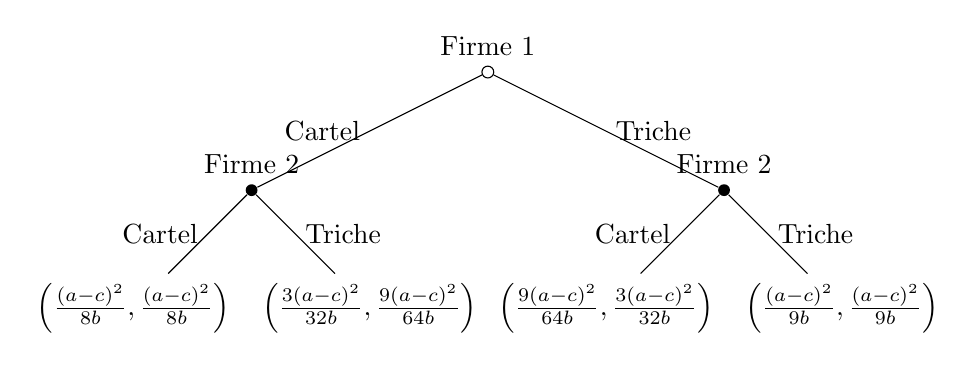
\begin{tikzpicture}[thin,
     level 1/.style={sibling distance=60mm},
     level 2/.style={sibling distance=30mm},
     level 3/.style={sibling distance=15mm},
     every circle node/.style={minimum size=1.5mm,inner sep=0mm}]
     
     \node[circle,draw,label=above: Firme 1] (root) {}
       child { node [circle,fill,label=above: Firme 2] {}
         child { 
           node {$\left(\frac{(a-c)^2}{8b}, \frac{(a-c)^2}{8b}\right)$}
           edge from parent
             node[left] {Cartel}}
         child { 
           node {$\left(\frac{3(a-c)^2}{32b}, \frac{9(a-c)^2}{64b}\right)$}
           edge from parent
             node[right] {Triche}}
         edge from parent
           node[left] {Cartel}}
       child { node [circle,fill,label=above: Firme 2] {}
       child { 
        node {$\left(\frac{9(a-c)^2}{64b},\frac{3(a-c)^2}{32b}\right)$}
        edge from parent
          node[left] {Cartel}}
          child { 
            node {$\left(\frac{(a-c)^2}{9b}, \frac{(a-c)^2}{9b}\right)$}
            edge from parent
              node[right] {Triche}}
          edge from parent
            node[right] {Triche}};
   \end{tikzpicture}
   \end{center}
   \caption{Représentation de la concurrence à la Cournot sous forme extensive}
 \end{figure}
    \end{itemize}
\end{frame}

\begin{frame}[allowframebreaks]{Répétition du jeu}
    \begin{itemize}
        \item Supposons que le jeu se répète deux fois: la firme $i$ choisit 
        la quantité $q_{it}$ à la période $t$, pour $i=1, 2$, et $t=1, 2$.
        \item \textbf{\underline{Quel est l'équilibre en sous-jeu parfait?}} 
        \item On résout le jeu(par induction) à rebours:
        \begin{enumerate}[-]
            \item En $t=2$ l'unique équilibre de Nash est $(triche, triche)$.
            \item En $t=1$ l'unique équilibre de Nash est $(triche, triche)$.
            \item Par conséquent, l'unique équilibre en sous-jeux parfait est $\left( 
                (triche, triche), (triche, triche)
            \right)$.
        \end{enumerate}
        \item \textbf{\underline{Autres questions}} : 
        \begin{enumerate}[-]
         \item qu'en est-il de $\left((cartel,cartel), (cartel,cartel)\right)$? 
         \item qu'en est-il de $\left((cartel, triche), (cartel, triche)\right)$?
         \item qu'en est-il de: la firm 1 joue $(cartel; triche \ \text{si} \ triche, cartel  \ \text{si} \ cartel)$,
          et la firme 2 joue $(cartel; triche \ \text{si} \ triche, cartel  \ \text{si} \ cartel)$?
        \item du jeu à 3,..., $N$ périodes?
\end{enumerate}
\end{itemize}
\end{frame}

\section{Jeu/concurrence à la Cournot infiniment répété}
\frame{\sectionpage}

\begin{frame}[allowframebreaks]{Actualisation}
\begin{itemize}
    \item Le jeu se répète un nombre infini de fois et on se demande 
    s'il existe des équilibre en sous-jeu parfait où les firmes jouent $cartel$
     toutes les deux à chaque fois?
     \item Pour y répondre on a besoin du concept d'actualisation:
     \begin{enumerate}[-]
         \item Le taux d'actualisation $\delta \in [0, 1]$, mesure "l'impatience" de la firme.
         \item Par exemple, la valeur actualisée de  $10$ euros reçus aujourd'hui et demain 
         est $10 + \delta 10$.
         \item Si $\delta = 1$, il n'y a pas de différence entre recevoir $10$ euros aujourd'hui et les 
         recevoir demain.
         \item On peut poursuivre le raisonnement avec  10 euros reçus aujourd'hui, demain, et après-demain, soit
         $10 + \delta 10 + \delta^2 10$, raisonnement que l'on peut encore poursuivre \ldots à l'infini.
         \item En fait, il s'agit d'une \textbf{série géométrique}. Elle a notamment la propriété:
         \begin{align*}
             \sum_{k = 0}^\infty \delta^k x &= \frac{x}{1-\delta}.
         \end{align*}
     \end{enumerate}
\end{itemize}
\end{frame}

\begin{frame}[allowframebreaks]{Cournot infiniment répété}
\begin{itemize}
    \item On note comme précédemment $q^{ca}_i$ la quantité de cartel pour la firme $i$(maximisant le profit des deux firmes), et $q_i^*$ 
    la quantité en concurrence à la Cournot.
    \item Nous avons le résultat suivant:  
    \begin{proposition}
        Si le taux d'actualisation $\delta$ est "suffisamment"  élevé 
         alors les stratégies suivantes constituent des équilibre de sous-jeu parfaits pour  
         le jeu de Cournot infiniment répété:  
         \begin{enumerate}[(a)]
             \item En $t$, la firme $i$ joue  $q_{it} =q^{ca}_i$ si $q_{j,t-1} =q^{ca}_j$ pour $j=1$ et $j=2$. 
             \item Jouer $q^*_i$ si $q_{j,t-1} \neq q^{ca}_j$ pour soit $j=1$ ou $j=2$.
         \end{enumerate}
    \end{proposition}
    \item La firme $i$ coopère tant que $j$ coopère.
    \item Une fois que $j$ triche $i$ produit la quantité d'équilibre de Nash-Cournot 
    pour toutes les périodes suivantes: \textbf{Nash reversion}.
    \item “Grim strategy”: pas de deuxième chance.
    \item Pour démontrer que ces strategies constituent des équilibres en sous-jeu parfaits il   
    faut obtenir des conditions qui "prescrivent" que la meilleure réponse 
    de la firme $i$ étant donné celle de la firme $j$ est aussi la meilleure réponse 
    dans chaque sous-jeu.
\end{itemize}

\end{frame}

\begin{frame}[allowframebreaks]{Éléments de démonstration}
\begin{itemize}
    \item Pour la firme $i=1, 2$, deux types de sous-jeu sont à considérer:
    \item \textbf{\underline{Sous-jeu de type 1}}:
    Après une période où un des joueurs à triché (dont soit $i$, ou $j=1, 2$, $i\neq j$):
    \begin{enumerate}[-]
        \item La stratégie proposée indique de jouer $q_i^*$ pour toujours étant donné que $j$ joue aussi 
        cette stratégie.  
        \item C'est un équilibre de Nash du sous-jeu: jouer "$q_i^*$ pour toujours" est la meilleure 
        réponse à la stratégie de $j$ de jouer "$q_j^*$ pour toujours".
        \item Ceci vérifie les critères d'un équilibre de sous-jeu parfait.
    \end{enumerate}
    \framebreak
    \item \textbf{\underline{Sous-jeu de type 2}}: Après une période sans triche.
    \begin{enumerate}[-]
        \item La stratégie proposée indique de coopérer et jouer $q_i^{ca}$, avec le profit actualisé de $\frac{\pi_i^{ca}}{1-\delta}$
        \item La meilleure stratégie alternative est de jouer $q_i^{mr}(q_j^{ca}) =: q_i^d$ à la période en cours,
         mais ceci entraîne $q_j =  q_j^*$ pour toujours. Le profit actualisé est ici 
         $\pi^d_i + \delta\left(\frac{\pi_i^*}{(1-\delta)}\right)$.
         \item Pour que $q_i^{ca}$ soit un équilibre de Nash de ce sous-jeu, il est nécessaire que,
         \begin{align*}
            \underbrace{\frac{\pi_i^{ca}}{1-\delta}}_{\text{profits sous coopération}} &> \underbrace{\pi^d_i + \delta\left(\frac{\pi_i^*}{(1-\delta)}\right)}_{\text{profits sous déviation/triche}}\\
            &\Rightarrow \delta >\frac{9}{17}.
         \end{align*}
    \end{enumerate}
    \item Par conséquent, la \textbf{Nash reversion} indique une meilleure réponse dans ces deux sous-jeux 
    si est "suffisamment élevé" avec $\delta >\frac{9}{17}$. 
    \item Dans ce cas la \textbf{Nash reversion} constitue un équilibre de sous-jeu parfait.
\end{itemize}
\end{frame}
\end{document}